\documentclass[12pt]{article}

\usepackage[utf8]{inputenc} % Required for inputting international characters
\usepackage[T1]{fontenc} % Output font encoding for international characters
\usepackage{mathpazo} % Palatino font


%%% PAGE DIMENSIONS
\usepackage[margin=2.54cm]{geometry} % 1.27 is narrower!
\geometry{a4paper} 

%%% Font set to times new roman
\usepackage{times}
%%% Really good graphics package
\usepackage{graphicx}

% Insert {PDFS}
\usepackage{pdfpages}

% Change section spacing, remove the spacing
\usepackage[compact]{titlesec}
\titlespacing*{\section}{0pt}{*0}{*0}
\titlespacing*{\subsection}{0pt}{*0}{*0}
\titlespacing*{\subsubsection}{0pt}{*0}{*0}

%%% Better floats
\usepackage{float}


\usepackage{tikz}
\usepackage{wrapfig}

%%% PACKAGES
\usepackage{booktabs} % for much better looking tables
\usepackage{amsmath} % for better maths
\usepackage{paralist} % very flexible & customisable lists (eg. enumerate/itemize, etc.)
\usepackage{verbatim} % adds environment for commenting out blocks of text & for better verbatim
\usepackage{subfig} % make it possible to include more than one captioned figure/table in a single float
\usepackage{mathtools} % matrices
\usepackage{blkarray, bigstrut} % matrices

\usepackage[framed,numbered]{matlab-prettifier} % enable inserting matlab code.
\usepackage[parfill]{parskip}
%\addtolength{\jot}{1em}
\usepackage{amssymb}
\usepackage{cancel}
\usepackage{color}
\usepackage{listings}
\usepackage{pdflscape} % Enabling rotating pages into a landscape orientation.


%%% HEADERS & FOOTERS
\usepackage{fancyhdr} % This should be set AFTER setting up the page geometry
\pagestyle{fancy} % options: empty , plain , fancy
\renewcommand{\headrulewidth}{0pt} % customise the layout...
\lhead{}\chead{}\rhead{}
\lfoot{}\cfoot{\thepage}\rfoot{}

%%% SECTION TITLE APPEARANCE
\usepackage{sectsty}
\renewcommand{\thesubsection}{\thesection.\alph{subsection}}

%%% ToC (table of contents) APPEARANCE
\usepackage[nottoc,notlof,notlot]{tocbibind} % Put the bibliography in the ToC
\usepackage[titles,subfigure]{tocloft} % Alter the style of the Table of Contents
\renewcommand{\cftsecfont}{\rmfamily\mdseries\upshape}
\renewcommand{\cftsecpagefont}{\rmfamily\mdseries\upshape} % No bold!

%%% Hyperlinking 
\usepackage{hyperref}
\begin{document}

\begin{titlepage} % Suppresses displaying the page number on the title page and the subsequent page counts as page 1
	\newcommand{\HRule}{\rule{\linewidth}{0.5mm}} % Defines a new command for horizontal lines, change thickness here
	\center % Centre everything on the page
	
	%------------------------------------------------
	%	Headings
    %------------------------------------------------
    
	\textsc{\LARGE 2019}\\[1.5cm] % Main heading such as the name of your university/college
	\textsc{\Large Semester 1}\\[0.5cm] % Major heading such as course name
	% \textsc{\large Department of Engineering Science}\\[0.5cm] % Minor heading such as course title
	
	%------------------------------------------------
	%	Title
	%------------------------------------------------
	
	\HRule\\[0.4cm]
	{\huge\bfseries ENGSCI 760 --- Assignment 1}\\[0.4cm] % Title of your document
	\HRule\\[1cm]
	
	%------------------------------------------------
	%	Author(s)
	%------------------------------------------------
	
    \begin{minipage}[t]{0.4\textwidth}
        \vspace{0pt}
		\begin{center}
			\large
			Noel \textsc{D'Souza}\\ % Your name
			\textit{ndso092}\\
			\textit{449609993}
		\end{center}
	\end{minipage}
	~
    % \begin{minipage}[t]{0.4\textwidth}
    %     \vspace{0pt}\raggedright
	% 	\begin{flushright}
	% 		\large
	% 		\textit{Employer Details}\\
    %         PwC \textsc{New Zealand} % Supervisor's name
    %         \linebreak \linebreak
    %         PwC Tower\\
    %         Level 22, 188 Quay St\\
    %         Auckland, 1010
	% 	\end{flushright}
	% \end{minipage}

	% If you don't want a supervisor, uncomment the two lines below and comment the code above
	%{\large\textit{Author}}\\
	%John \textsc{Smith} % Your name
	
	%------------------------------------------------
	%	Date
	%------------------------------------------------
	
	\vfill\vfill\vfill % Position the date 3/4 down the remaining page
	
    {\large\today} % Date, change the \today to a set date if you want to be precise
    % {\large 7 August, 2019}
	
	%------------------------------------------------
	%	Logo
	%------------------------------------------------
	
    % \vfill
    
    % \begin{minipage}[t]{0.4\textwidth}
    %     \vspace{0pt}
    %     \begin{flushleft}
    %     \includegraphics[width=0.9\textwidth]{engtitle.png}\\[1cm]
	% 	\end{flushleft}
	% \end{minipage}
	% ~
    % \begin{minipage}[t]{0.4\textwidth}
    %     \vspace{0pt}\raggedright
	% 	\begin{flushright}
    %         \includegraphics[width=0.45\textwidth]{pwc.png}\\[1cm]        
	% 	\end{flushright}
	% \end{minipage}


    % \includegraphics[width=0.4\textwidth]{engtitle.png}\\[1cm] % Include a department/university logo - this will require the graphicx package
	 
	%----------------------------------------------------------------------------------------
	
	\vfill % Push the date up 1/4 of the remaining page
	
\end{titlepage}

%------------------------------------------------
%   Summary
%------------------------------------------------

\section{Joint Distributions}

\subsection{Pairwise Independence?}

Events A, B and C \textbf{are} pairwise independent since the outcomes in any \textbf{pair of events} are independent of each other.
\begin{align*}
P(A\cap B) &= P(A)P(B) = \frac{1}{36}\\
P(B\cap C) &= P(B)P(C) = \frac{1}{36}\\
P(A\cap C) &= P(A)P(C) = \frac{1}{36}\\
\end{align*}

\subsection{Mutual indepentence?}

Events A, B and C \textbf{are not} mutually independent. If we know the outcome of Events B and C, then we know, with 100\% certainty, the outcome of Event A. In other words, Event A is \textbf{dependent} on the intersection of Events B and C.
\begin{align*}
	P(A|\{B\cap C\}) &= 1\\
	\text{Hence } P(A\cap B\cap C) &\neq P(A)P(B)P(C)
\end{align*}


\section{Markov Chains}

\subsection{One-Step Transition Matrix}
\begin{equation*}
	\mathbf{P}=
	\begin{blockarray}{*{5}{c} l}
	  \begin{block}{*{5}{>{$\footnotesize}c<{$}} l}
		U & G & A & P & S & \\
	  \end{block}
	  \begin{block}{[*{5}{c}]>{$\footnotesize}l<{$}}
		0 & 0.4 & 0.3 & 0.2 & 0.1 \bigstrut[t]& U \\
		0 & 1 & 0 & 0 & 0 & G \\
		0 & 0 & 1 & 0 & 0 & A \\
		0 & 0.4 & 0.3 & 0.2 & 0.1 & P \\
		0 & 0 & 0 & 0 & 1 & S \\
	  \end{block}
	\end{blockarray}
\end{equation*}

\subsection{Limiting Distributions}
	
\begin{align*}
	\text{Proportion of good items} & = \text{Probability that a given item is good} \\
	& = \text{Pr(item reaches G in step 1 \textit{or} item reaches G in step 2 \textit{or} ...)} \\
	& = \text{Pr(item good in step 1) + Pr(item good in step 2) + ...}\\
	& = 0.4 + (0.2)(0.4) + (0.2)(0.2)(0.4) + (0.2)(0.2)^2(0.4) + ... \\
	& = 0.4 + (0.2)(0.4)\sum_{k=0}^{\infty}{(0.2)^k}\\
	& = 0.4 + \frac{0.08}{0.8}\\
	\text{Pr}(X_t = \text{G})& = 0.5
\end{align*}

\begin{align*}
	\text{Proportion of average items} & = \text{Pr(average in step 1) + Pr(average in step 2) + ...}\\
	& = 0.3 + (0.2)(0.3) + (0.2)(0.2)(0.3) + (0.2)(0.2)^2(0.3) + ... \\
	& = 0.3 + (0.2)(0.3)\sum_{k=0}^{\infty}{(0.2)^k}\\
	& = 0.3 + \frac{0.06}{0.8}\\
	\text{Pr}(X_t = \text{A})& = 0.375\\
&\\
	\text{Proportion of scrapped items} & = \text{Pr(scrap in step 1) + Pr(scrap in step 2) + ...}\\
	& = 0.1 + (0.2)(0.1) + (0.2)(0.2)(0.1) + (0.2)(0.2)^2(0.1) + ... \\
	& = 0.1 + (0.2)(0.1)\sum_{k=0}^{\infty}{(0.2)^k}\\
	& = 0.1 + \frac{0.02}{0.8}\\
	\text{Pr}(X_t = \text{S})& = 0.125\\
	& \\
	\text{Pr}(X_t = \text{U}) &= \text{Pr}(X_t = \text{P}) = 0
\end{align*}
\newline
\subsection{Expected Profit From Unfinished Item}

\begin{align*}
\text{Note that:}\\
m_{ij} & = \sum_{k=1}^{n} p_{ik}(m_{kj}+1) \text{, where } i \neq j\\
& = 1 + \sum_{k=1}^{n} p_{ik}m_{kj} \text{, where } i \neq j\\
& \\
m_{\text{UG}} &= 1 + p_{\text{UU}}m_{\text{UG}} + p_{\text{UG}}m_{\text{GG}} + p_{\text{UA}}m_{\text{AG}} + p_{\text{UP}}m_{\text{PG}} + p_{\text{US}}m_{\text{SG}}\\
&= 1 + (0)m_{\text{UG}} + (0.4)m_{\text{GG}} + (0.3)m_{\text{AG}} + (0.2)m_{\text{PG}} + (0.1)m_{\text{SG}}\\
& = 1 + 0 + (0.4)(0) + (0.3)(0) + 0.2m_{\text{PG}} + (0.1)(0)\\
& = 1 + 0.2m_{\text{PG}}\\
& \\
\text{Similarly:}\\
m_{\text{UA}} &= 1 + 0.2m_{\text{PA}}\\
m_{\text{US}} &= 1 + 0.2m_{\text{PS}}\\
& \\
\end{align*}
Note that $m_{\text{U}i}$ $=$ $m_{\text{P}i}$ as per the transition probabilities hence we can rearrange the above:
\begin{align*}
m_{\text{UG}} &= 1 + 0.2m_{\text{UG}}\\
m_{\text{UA}} &= 1 + 0.2m_{\text{UA}}\\
m_{\text{US}} &= 1 + 0.2m_{\text{US}}\\
& \\
\text{Therefore all paths have the same mean hitting time:}\\
m_{\text{UG}} &= m_{\text{UA}} = m_{\text{US}} = 1.25\\
& \\
\text{Expected profit} & = (50\times0.5) + (40\times0.375) - (10\times1.25) - 20\\
& = \$7.50
\end{align*}

\subsection{Updated One-Step Transition Matrix}
\begin{equation*}
	\mathbf{P_{new}}=
	\begin{blockarray}{*{6}{c} l}
	  \begin{block}{*{6}{>{$\footnotesize}c<{$}} l}
		U & G & A & S & $P_1$ & $P_2$ & \\
	  \end{block}
	  \begin{block}{[*{6}{c}]>{$\footnotesize}l<{$}}
		0 & 0.4 & 0.3 & 0.1& 0.2 & 0\bigstrut[t]& U \\
		0 & 1 & 0 & 0 & 0 & 0 & G \\
		0 & 0 & 1 & 0 & 0 & 0 & A \\
		0 & 0 & 0 & 1 & 0 & 0 & S \\
		0 & 0.4 & 0.3 & 0.1 & 0 & 0.2 & $P_1$ \\
		0 & 0.4 & 0.3 & 0.3 & 0 & 0 & $P_2$ \\
	  \end{block}
	\end{blockarray}
\end{equation*}

\section{Hidden Markov Model}

Note: Code is attached as an appendix\newline

\textbf{The Intended Message:}\newline
could you order a peri peri chicken sandwich for me and fries for alice\newline
we want you to go to the closest restaurant\newline
are you driving there in your car\newline
where are you\newline
how far are you from here\newline
we are starving\newline
what time will you show up here\newline

\section{Decision Analysis}
\subsection{Beysian Network}
\includepdf[pages=-]{Beysian-network}

\subsection{Decision Tree}
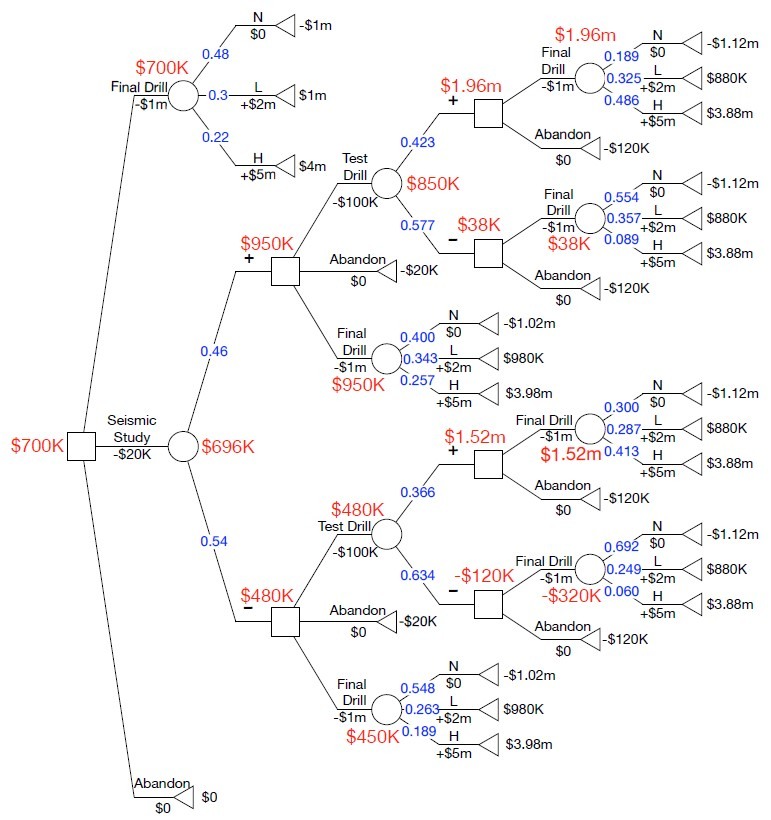
\includegraphics[scale=0.8]{Decision-tree.jpg}
Probabilities rounded to 3dp
% \includepdf[pages=-]{decision-tree}
\subsection{Decisions decisions...}
Assuming Anadarko is risk-neutral, the optimal strategy is to drill the final well immediately---with an expected profit of \$700K. This is greater than that from seismic testing and drilling test drills (\$696K), or abandoning the site (\$0).

Assuming Anadarko is very risk-averse, the optimal strategy would be to conduct seismic testing (and potentially drill test wells later). This hasan expected profit that is only \$4,000 lower than drilling the final well immediately. Even though the expected profit is lower, Anadarko can minimise potential losses by retaining the option of abandoning the site at any point before drilling the final well.

\newpage

\section{Appendix}
\subsection{HMMfinal.py}
\lstinputlisting[language=Python]{HMMfinal.py}
\newpage
\subsection{beliefprop.py}
\lstinputlisting[language=Python]{beliefprop.py}



\end{document}
